\documentclass[12pt,letterpaper]{article}
\usepackage[utf8]{inputenc}
\usepackage[spanish,USenglish]{babel}
\usepackage{amsmath,amsfonts,amssymb,amsthm}
\usepackage{graphicx}
\usepackage{epsfig}
\usepackage{setspace}
\usepackage{enumerate} 
%gráficos y figuras
\usepackage{pgf,tikz,pgfplots}
\usetikzlibrary{arrows}
\pgfplotsset{compat=1.15}
\usetikzlibrary{trees,arrows,positioning,calc}
\tikzstyle{redVertex}  =[draw,fill=red,circle,minimum size=30pt,inner sep=-0pt, text=white]
\tikzstyle{blackVertex}=[draw,fill=black,circle,minimum size=30pt,inner sep=0pt, text=white]
\tikzstyle{nil}=[draw,fill=black,rectangle,minimum size=30pt,inner sep=0pt, text=white]
%escribir programas
\usepackage{listings}
%encabezado
\usepackage{fancyhdr}
\pagestyle{fancy}
\fancyhf{}
% Números de página en las esquinas de los encabezados
\fancyhead[R]{\thepage} 
%Espacio para Titulo (revisar warnings)
\setlength{\headheight}{14.5pt}
% Formato para la sección: N.M. Nombre
\renewcommand{\sectionmark}[1]{\markright{\textbf{\thesection. #1}}{}} 
%título
\title{ \textbf{Tarea Uno} \\ Optimización I}
\author{Esteban Reyes Saldaña}
\date{\today}
%definiciones
\theoremstyle{definition}
\newtheorem{problm}{Problema}
\usepackage{colortbl}
\usepackage{tabularx}
\usepackage{dcolumn}
\usepackage{multirow}
\usetikzlibrary[patterns]

\begin{document}
	
\selectlanguage{spanish}
\maketitle 
\begin{problm}
	Sea $ f_1(x_1, x_2) = x_1^2 - x_2^2 $, $ f_2(x_1, x_2) = 2x_1 x_2 $. Represente los conjuntos de nivel asociados con $ f_1(x_1, x_2) = 12 $ y $ f_2(x_1, x_2) = 16 $ sobre la misma figura usando Python. Indique sobre la figura los puntos $ \textbf{x} = \left[ x_1, x_2 \right]^T $ para los cuales $ f(\textbf{x}) =  \left[f_1(x_1, x_2), f_2(x_1, x_2)\right]^T = \left[12, 16 \right]^T $.
	\\
	\textbf{Solución} la gráfica obtenida fue
	\begin{center}
		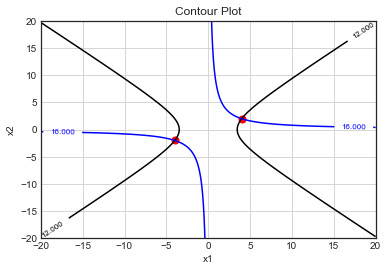
\includegraphics[width=0.7\linewidth]{contour}
	\end{center}
	(Parte analítica). Dadas las ecuaciones
	\begin{eqnarray}\label{sistema}
		\left\{\begin{matrix}
			x_1^2 - x_2^2 & = & 12 \\
			2x_1 x_2      & = & 16.
		\end{matrix}\right.
	\end{eqnarray}
	Como $ x_1 x_2 = 8 $, entonces tanto $ x_1 $ como $ x_2 $ son distintos de cero. Luego, de la segunda ecuación tenemos que
	\begin{equation}\label{equisdos}
		x_2 = \dfrac{8}{x_1}.
	\end{equation}
	Así que la primera ecuación se puede reescribir como
	\begin{eqnarray*}
		x_1^2 - \left( \dfrac{8}{x_1} \right)^2 & = & 12 \\
		x_1^2 - \dfrac{64}{x_1^2} 				& = & 12.		
	\end{eqnarray*}
	Sea $ u = x_1^2 $, entonces
	\begin{eqnarray*}
		u - \dfrac{64}{u} & = & 12 \\
		\dfrac{u^2 - 64}{u} & = & 12 \\
		u^2 -64 & = & 12u	         \\
		u^2 - 12u -64 & = & 0.
	\end{eqnarray*}
	Resolviendo esta ecuación cuadrática obtenemos
	\[ u = \dfrac{12 \pm \sqrt{144 + 256}}{2} =  \dfrac{12 \pm 20}{2} \]
	Así que las soluciones para $ u $ son 
	\[ u = 16 \textup{ o } u = -4 \]
	Como $ x_1^2 = u \in\mathbb{R}^+ $ entonces obtenemos que $ x_1^2 = 16 $, de donde
	\[ x_1 = -4 \textup{ o } x_1 = 4. \]
	Finalmente, de la ecuación (\ref{equisdos}) obtenemos que las soluciones a (\ref{sistema}) son
	\[ (-4, -2) \textup{ o }  (4, 2). \]
\end{problm}

\begin{problm}
	Considere la función $ f(x) = (a^T x) (b^T x) $, donde $ a, b $ y $ x $ son vectores $ n $- dimensionales. Calcule el gradiente $ \nabla f(x) $ y el Hessiano $ \nabla^2 f(x) $.
	\\
	\textbf{Solución}. Sabemos que
	\[ D f(x) = \nabla f(x)^T . \]
	y que para dos vectores $ a, b \in\mathbb{R}^n$ se tiene que
	\begin{equation}\label{1}
		<a,b> = a b^T = b a^T
	\end{equation}
	Así que usando la regla del producto para derivadas obtenemos
	\begin{eqnarray*}
		D_x (a^T x) (b^T x) & = & (a^T x) D _x (b^T x) +  (b^T x) D_x (a^T x) \\
		 					& = & (a^T x) b^T +  (b^T x) a^T \\
						    & = & a^T x b^T + b^T x a^T \\
						    & = & \underbrace{x^T a b^T + x^T b a^T}_{(\ref{1})} \\
						    & = & x^T (ab^T + b a^T) \\
						    & = & \underbrace{(ab^T + b a^T) x^T}_{\textup{conmutatividad escalar-vector}}  \\
	\end{eqnarray*}
	Por lo que
	\begin{eqnarray*}
		\nabla f(x) & = & D_x ^T f(x) \\
					& = & \left[ (ab^T + b a^T) x^T \right]^T \\
					& = & (ab^T + b a^T) x.
	\end{eqnarray*}
	Ahora, dado que el gradiente de f resultó ser el producto de un escalar por el vector $ x $ tenemos que
	\begin{eqnarray*}
		\nabla^2 f(x) & = & \nabla (\nabla f(x)) \\
		   			  & = & \nabla ((ab^T + b a^T) x) \\
		   			  & = & D_x ((ab^T + b a^T) x)^T \\
		   			  & = & (ab^T + b a^T) D_x(x)^T \\
		   			  & = & (ab^T + b a^T).
	\end{eqnarray*}
\end{problm}

\begin{problm}
	Sea $ f(x) = \dfrac{1}{1+e^{-x}} $ y $ g(z) = f(a^T z + b) $ con $ ||a||_2 = 1 $. Demuestre que $ D_a g(z) = g(z) (1-g(z)) $.
	\begin{proof}
		Por un lado, tenemos que $ g: \mathbb{R}^n \mapsto \mathbb{R} $ y en clase se vió que
		\begin{equation}\label{2}
			D_a g(z) = \nabla g(x)^T a
		\end{equation}
	
	Por otro lado, sea $ h(z) = a^T z + b $, entonces
	\begin{equation}\label{ache}
		g(z) = f(h(z)).
	\end{equation}
	Observemos que
	\begin{eqnarray*}
		f'(x) & = & -\dfrac{1}{(1+e^{-x})^2} (-e^{-x}) \\
			  & = & \dfrac{1}{(1+e^{-x})^2} ( 1 + e^{-x} - 1) \\
			  & = & \dfrac{1 + e^{-x}}{(1+e^{-x})^2} - \dfrac{1}{(1+e^{-x})^2} \\
			  & = & \dfrac{1}{1+e^{-x}} - \left(\dfrac{1}{1+e^{-x}}\right)^2 \\
			  & = & f(x) - f^2(x) \\
			  & = & f(x) (1-f(x)).
	\end{eqnarray*}
	y
	\begin{eqnarray*}
		D_z(h(z)) & = & D_z(a^T z + b) \\
		 		 & = & D_z(a^Tz) + D_z(b) \\
		 		 & = & a^T.
	\end{eqnarray*}
	Ahora, de (\ref{2}) y por regla de la cadena tenemos que
	\begin{eqnarray*}
		 D_a g(z) & = & D f(h(z)) D (h(z)) a \\
		          & = & f(h(z)) (1-f(h(z))) a^T a.
	\end{eqnarray*}
	Por la forma en la que se definió $ h(z) $ en (\ref{ache}) y dado que $ a^T a = || a ||_2 = 1 $, se concluye que
	\begin{eqnarray*}
		D_a g(z) & = & f(h(z)) (1-g(h(z))) a^T a \\
				 & = & g(z) (1-g(z)).
	\end{eqnarray*}
	\end{proof}
\end{problm}

\begin{problm}
	Calcule el gradiente de
	\[ f(\theta) = \dfrac{1}{2} \sum_{t = 1}^{n} [g(x_i) - g(Ax_i + b)]^2 \]
	con respecto a $ \theta $, donde $ \theta = [a_{11}, a_{12}, a_{21}, a_{22}, b_1, b_2]^T $, $ x_i \in \mathbb{R}^2 $, $ A\in\mathbb{R}^{2 \times 2} $, $ b\in\mathbb{R}^2 $ están definidas como sigue
	\begin{eqnarray*}
		A & = & \left[\begin{matrix}
				a_{11} & a_{12} \\
				a_{21} & a_{22} 
			\end{matrix}\right]  \\
		b & = & [b_1 b_2]^T
	\end{eqnarray*}
	y $ g: \mathbb{R}^2 \to \mathbb{R} \in\mathcal{C}^1 $.
	\\
	\textbf{Solución.} Usando la relación entre gradiente-derivada y por regla de la cadena tenemos que
	\begin{eqnarray*}
		\nabla f(\theta)^T & = &  D_{\theta} \left( \dfrac{1}{2} \sum_{t = 1}^{n} [g(x_i) - g(Ax_i + b)]^2 \right) \\
						   & = & \dfrac{1}{2} 2 \sum_{t = 1}^{n} [g(x_i) - g(Ax_i + b)] D [g(x_i) - g(Ax_i + b)] \\
						   & = & \dfrac{1}{2} 2 \sum_{t = 1}^{n} [g(x_i) - g(Ax_i + b)] [D g(x_i) - D g(Ax_i + b)] \\
						   & = & \sum_{t = 1}^{n} [g(x_i) - g(Ax_i + b)] [D g(x_i) - D g(Ax_i + b)] \\
						   & = & \sum_{t = 1}^{n} [g(x_i) - g(Ax_i + b)] [0 - D g(Ax_i + b) D (A x_i + b)] \\
						   & = & - \sum_{t = 1}^{n} [g(x_i) - g(Ax_i + b)] D g(Ax_i + b) D(A x_i + b) \\ 
						   & = & - \sum_{t = 1}^{n} [g(x_i) - g(Ax_i + b)] D g(Ax_i + b) (D(A x_i) + D(b)).
	\end{eqnarray*}
\end{problm}

\begin{problm}
	Demuestre que $ \kappa(A) \geq 1 $ donde $ || A || = \max_{x} \dfrac{||Ax||}{||x||} $ (Sugerencia: demuestre que $ || AB || \leq || A || || B || $).
	\\
	\begin{proof}
		Primero se verá que $ || AB || \leq || A || || B || $. En efecto, para $ x\neq 0 $ tenemos que
		\begin{eqnarray*}
			|| A || & = & \max_{x} \dfrac{|| Ax ||}{|| x ||}
		\end{eqnarray*}
	y por la definición de máximo sobre $ x $ no nulo,
	\begin{eqnarray*}
		\dfrac{|| A x || }{|| x ||} & \leq  & || A || \\
		|| A x || & \leq & || A || ||x ||.
	\end{eqnarray*}
	Ahora, por la propiedad anterior se tiene que
	\begin{eqnarray*}
		|| A B || & = & \max_{x} \dfrac{|| A B x || }{|| x || } \\
		          & \leq & \max_{x} \dfrac{|| A || || B x || }{|| x ||} \\
		          & \leq & \max_{x} \dfrac{|| A || || B || ||x || }{|| x ||} \\
		          & = & \max_{x} || A || || B || \\
		          & = & || A || || B ||.		          
	\end{eqnarray*}
	\end{proof}
\end{problm}

\begin{problm}
	Demuestre que $ x - \sin(x) = o(x^2) $ cuando $ x \to 0 $.
	\\
	\begin{proof}
		Hay que demostrar que 
		\[ \lim_{x \to 0} \dfrac{x - sen(x) }{x^2} = 0. \]
		En efecto, procedemos aplicando la regla de L'Hospital. Si
		\begin{eqnarray*}
			f(x) & = & x - sen(x).\\
			g(x) & = & x^2
		\end{eqnarray*}
		tenemos que $ f(x), g(x) \in\mathcal{C}^{\infty} $ sobre $ \mathbb{R} $ con $ f(0)  = 0$ y $ g(0) = 0 $. Además,
		\begin{eqnarray*}
			f'(x) & = & 1 + cos(x)\\
			g'(x) & = & 2x
		\end{eqnarray*}
		y
		\begin{eqnarray*}
			f''(x) & = & -sen(x).\\
			g'(x) & = & 2
		\end{eqnarray*}
		donde $ f''(0) = 0 $ y $ g'''(0)  = 2 \neq 0 $, así que, por la regla de $ L'Hospital $, tenemos que
		\begin{eqnarray*}
			\lim_{x \to 0} \dfrac{x-sen(x)}{x^2} & = & \lim_{x \to 0} \dfrac{1+cos(x)}{2x} \\
												 & = & \lim_{x \to 0} \dfrac{-sen(x)}{2} \\
												 & = & 0.
		\end{eqnarray*}
	De lo anterior se concluye que $ x-sen(x) \in 0(x^2) $.
	\end{proof}
\end{problm}

\begin{problm}
	Suponga que $ f(x) = o (g(x)) $. Demuestre que para todo $ \epsilon > 0 $, existe $ \delta > 0 $ tal que si $ 0 < || x || < \delta $, entonces $ |f(x)| < \epsilon |g(x)| $, i.e, $ f(x) = O(g(x)) $ para $ 0 < || x || < \delta $.
	\\
	\begin{proof}
		Sin pérdida de generalidad, suponga que $ x \to 0 $ (de otro modo se considera una translación a cero). Supongamos que $ f(x) = o(g(x)) $ cuando $ x \to 0 $. Entonces
		\[ \lim_{x \to 0} \dfrac{f(x)}{g(x)} = 0 \]
		Por definición se tiene que, para todo $ \epsilon > 0 $ existe $ \delta > 0 $ para el cual si
		\[0 <||x|| < \delta \textup{ entonces } \left|\dfrac{f(x)}{g(x)}\right| < \epsilon.\]
		Además sabemos que como este límite existe, $ g(x) \neq 0 $ para $ 0 < || x || < \delta $. Entonces
		\[ |f(x)| < \epsilon |g(x)|. \]
		Es decir, $ f(x) = O(g(x)) $ para $ 0 < || x || < \delta $.
	\end{proof}
\end{problm}

\begin{problm}
	Demuestre que si las funciones $ f: \mathbb{R}^n \to \mathbb{R} $ y $ g : \mathbb{R}^n \to \mathbb{R} $ satisface $ f(x) = -g(x) + o(g(x)) $ y $ g(x) > 0 $ para todo $ x \neq 0 $, entonces para todo $ x \neq 0 $ suficientemente pequeño, se tiene que $ f(x) < 0 $.
	\begin{proof}
		Notemos que 
		\[ f(x) = -g(x) + o(g(x)) \]
		es equivalente a
		\[ f(x) + g(x) = o(g(x)). \]
		Por el problema anterior, sabemos que para todo $ \epsilon > 0 $, existe $ \delta > 0 $ tal que si $ 0 < || x || < \delta $ entonces 
		\[| f(x) + g(x) | < \epsilon | g(x) |\]
		Luego, como $ g(x) > 0 $ para todo $ x \neq 0 $, $ | g(x) | = g(x) $, entonces
		\begin{eqnarray}
			-\epsilon g(x) & <  f(x) + g(x) < & \epsilon g(x)
		\end{eqnarray}
		de donde
		\[ -(\epsilon+1) g(x) = -\epsilon g(x) - g(x) < f(x) < \epsilon g(x) - g(x) = (\epsilon - 1) g(x) \]
		Así que se elige $ 0 < \hat{\epsilon} < 1 $ entonces $ \hat{\epsilon} - 1 < 0 $ por lo que existe $ \hat{\delta} > 0 $ tal que si $ ||x|| < \hat{\delta} $ entonces
		\[ f(x) < (\hat{\epsilon} - 1) g(x) < 0. \]
		Es decir, $ f(x) < 0 $ para un $ x $ lo suficientemente pequeño
	\end{proof}
\end{problm}

\end{document}
